\documentclass[notitlepage]{report}

\usepackage{graphicx}
\usepackage{subfig}

\title{PA 1: Bloom Filter}
\author{David Johnston}

\begin{document}
\maketitle

\begin{abstract}
Hello, world!
\end{abstract}

\section{\texttt{FalsePositives}}

\begin{figure}[h]
  \makebox[\textwidth][c]{
    \subfloat[][$b=4$]{
      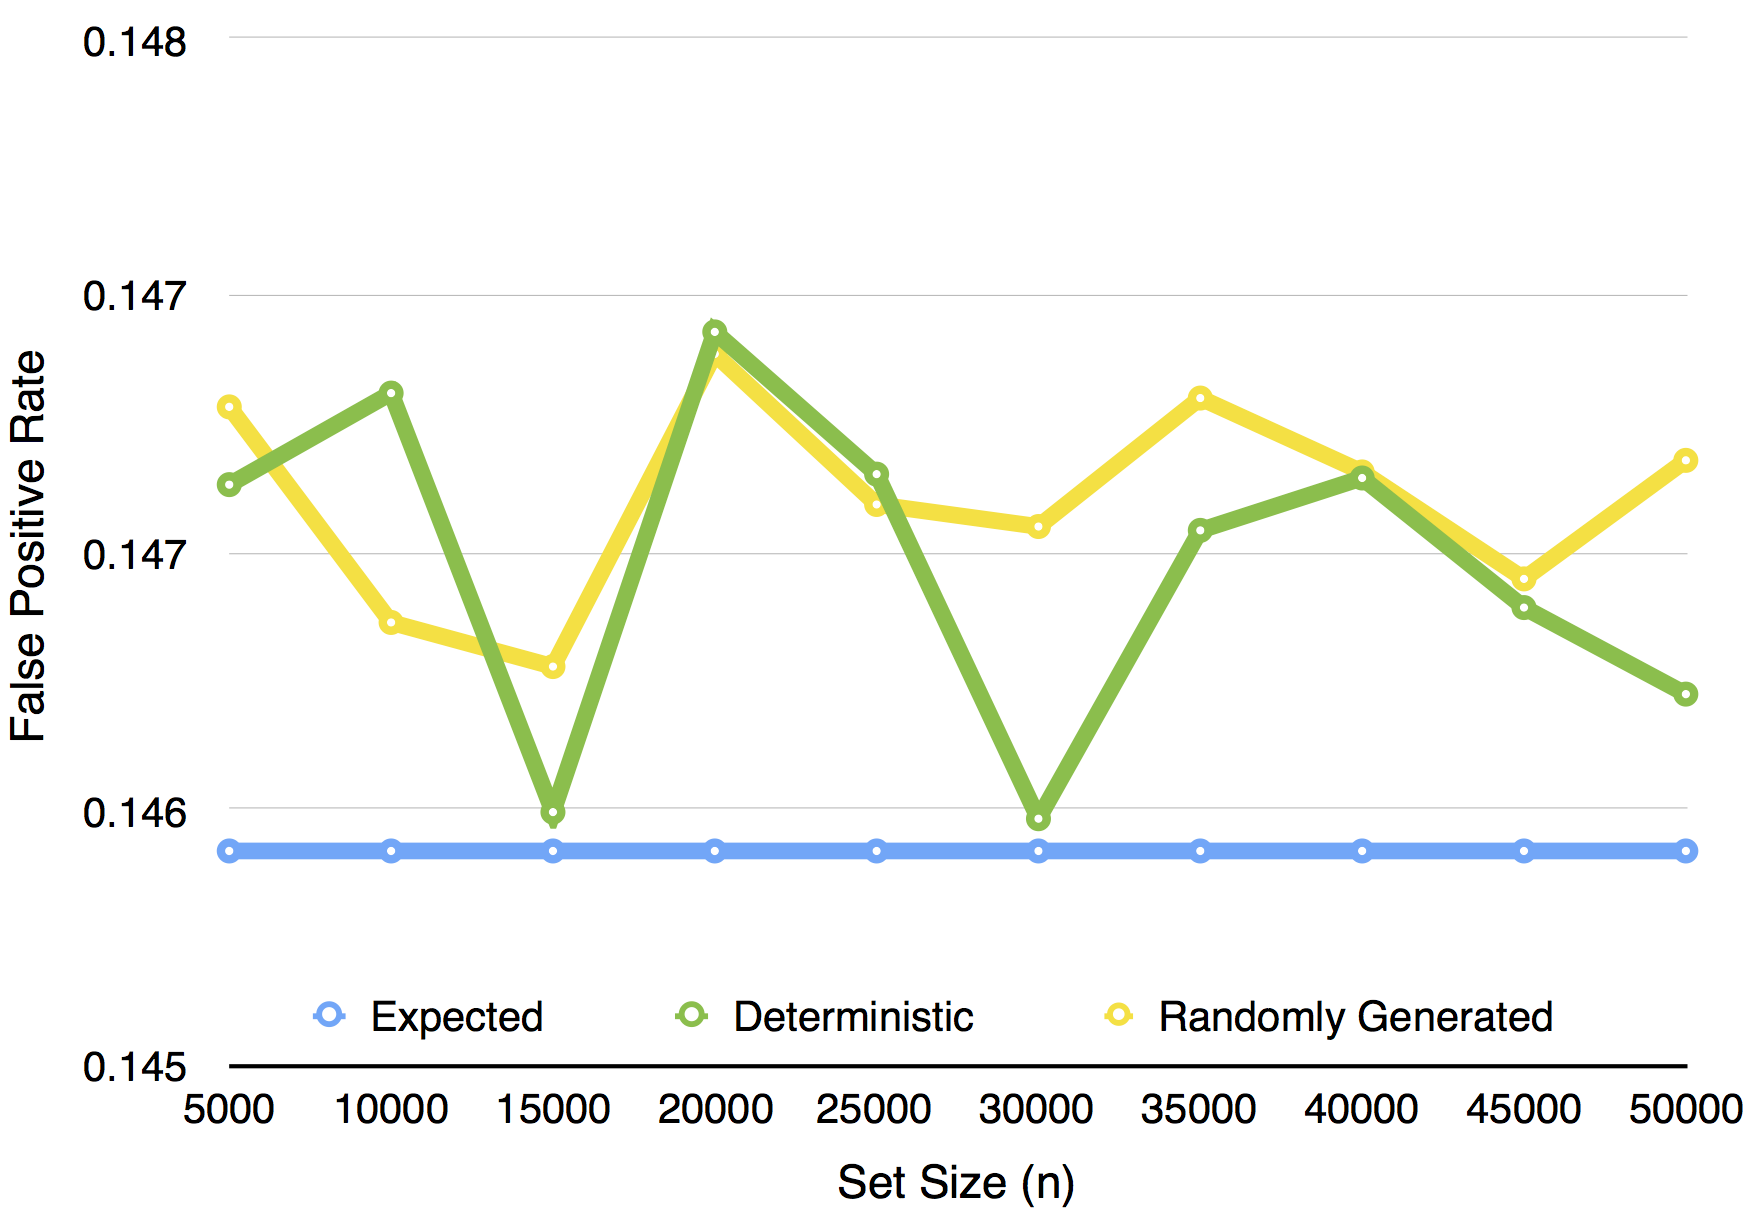
\includegraphics[width=0.5\textwidth]{figures/false_positives/b=4}
    }
    \subfloat[][$b=8$]{
      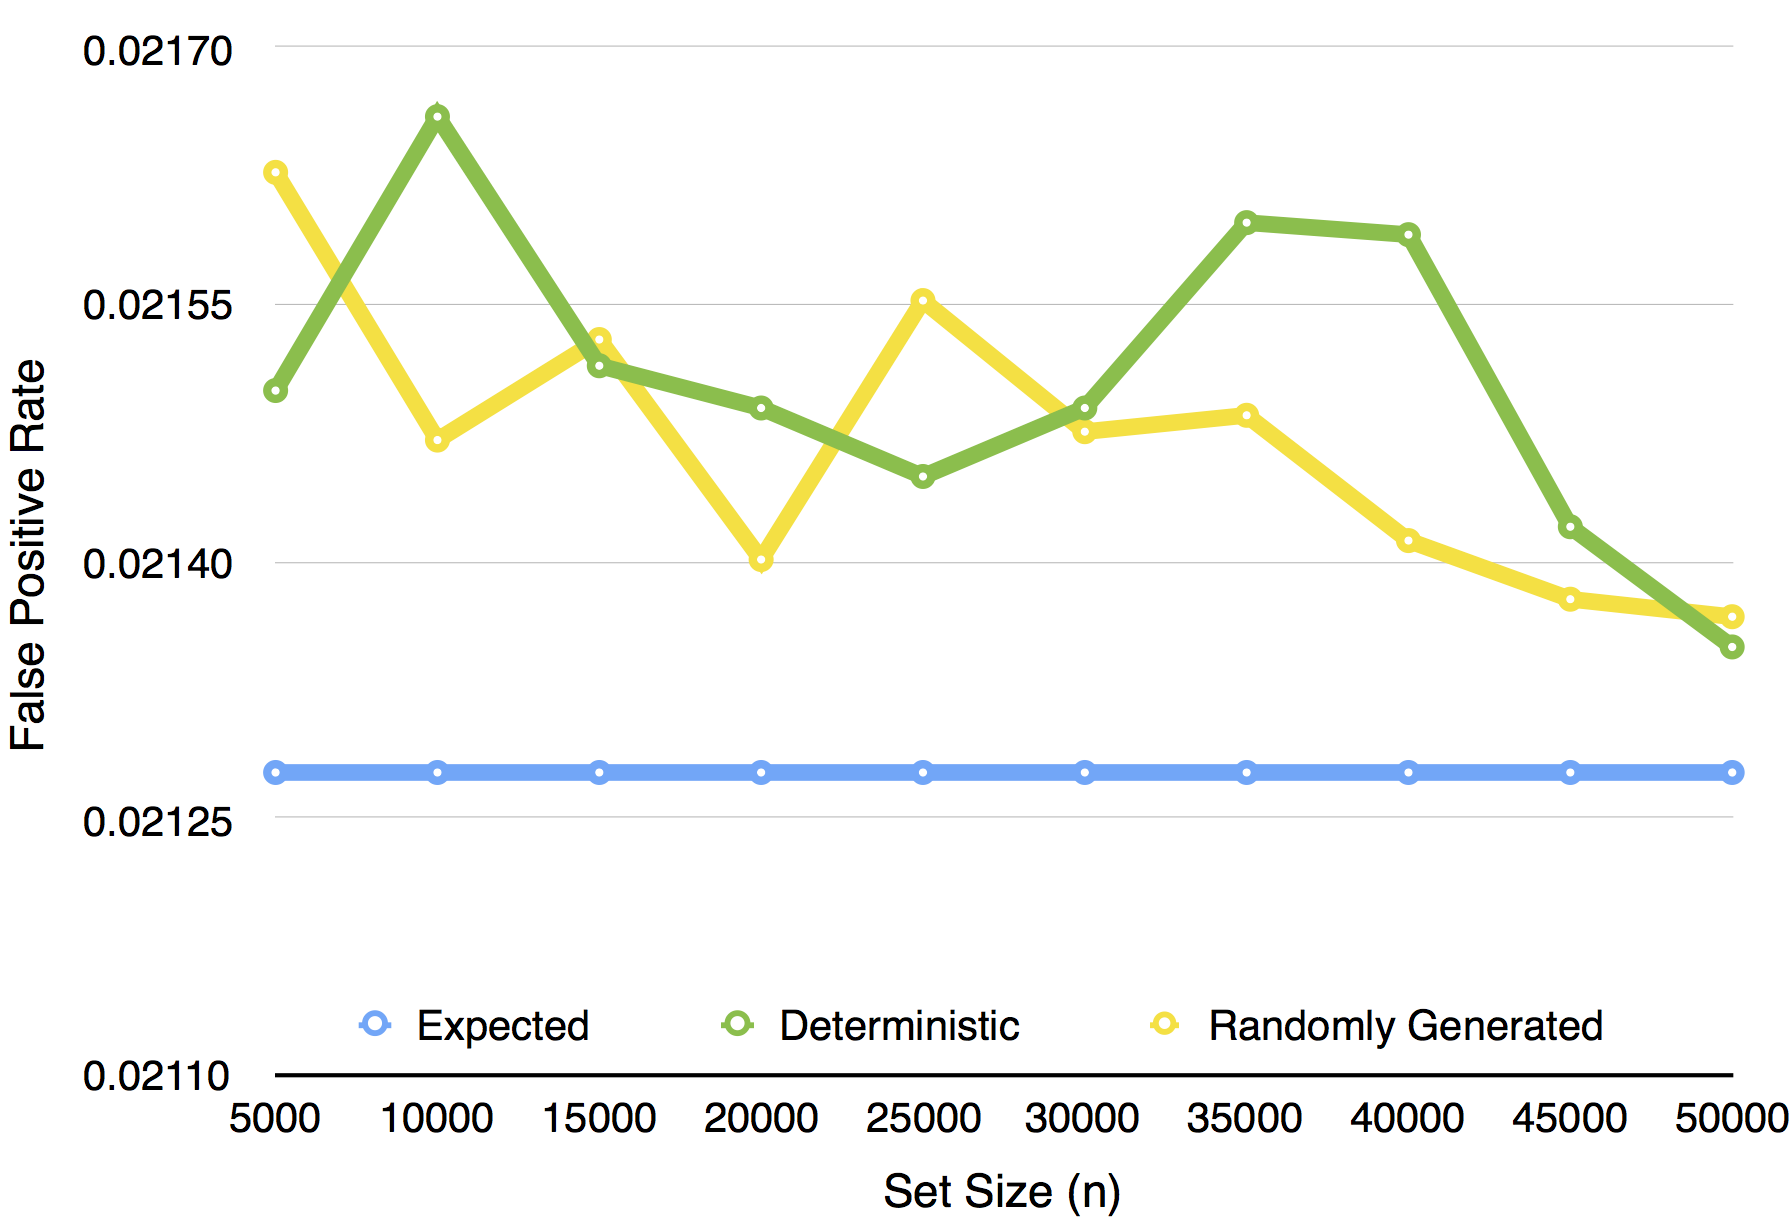
\includegraphics[width=0.5\textwidth]{figures/false_positives/b=8.png}
    }
  }

  \makebox[\textwidth][c]{
    \subfloat[][$b=12$]{
      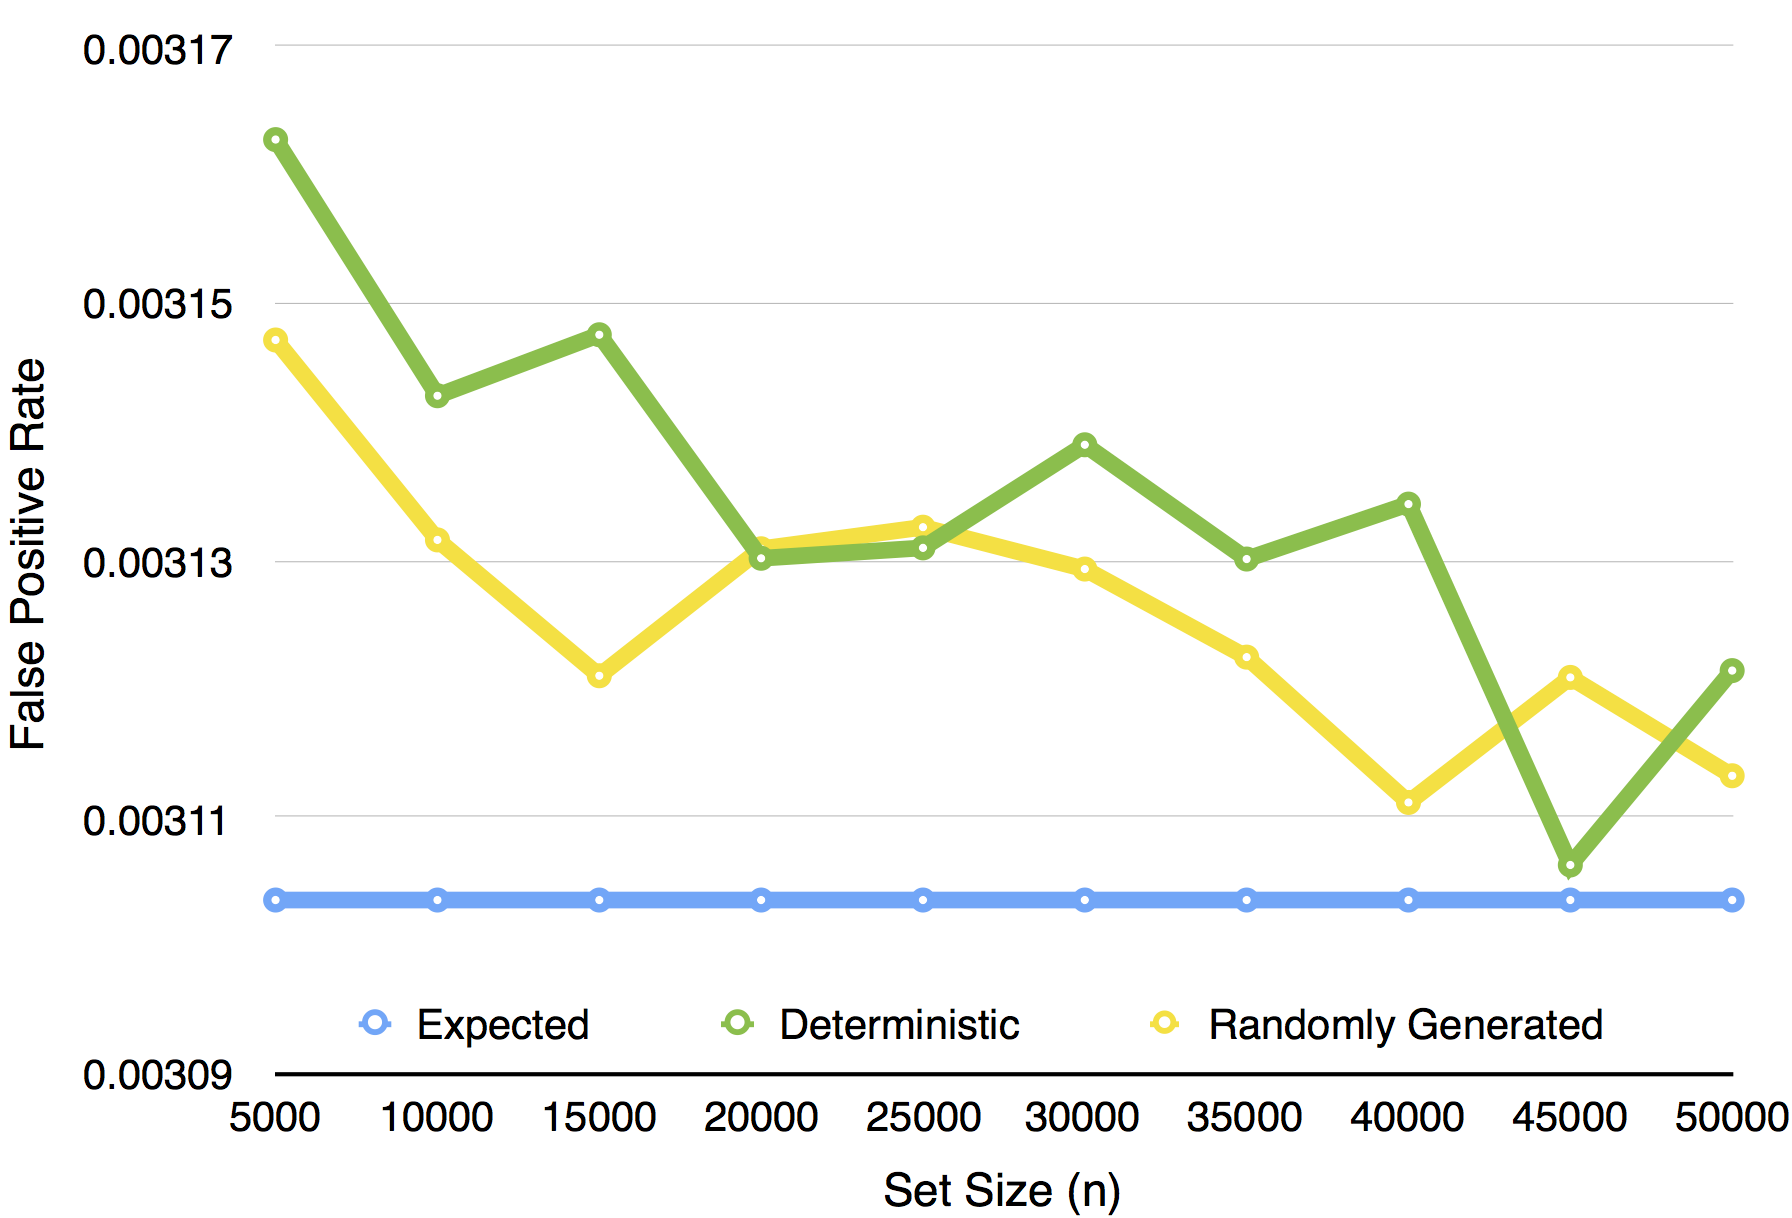
\includegraphics[width=0.5\textwidth]{figures/false_positives/b=12.png}
    }
    \subfloat[][$b=16$]{
      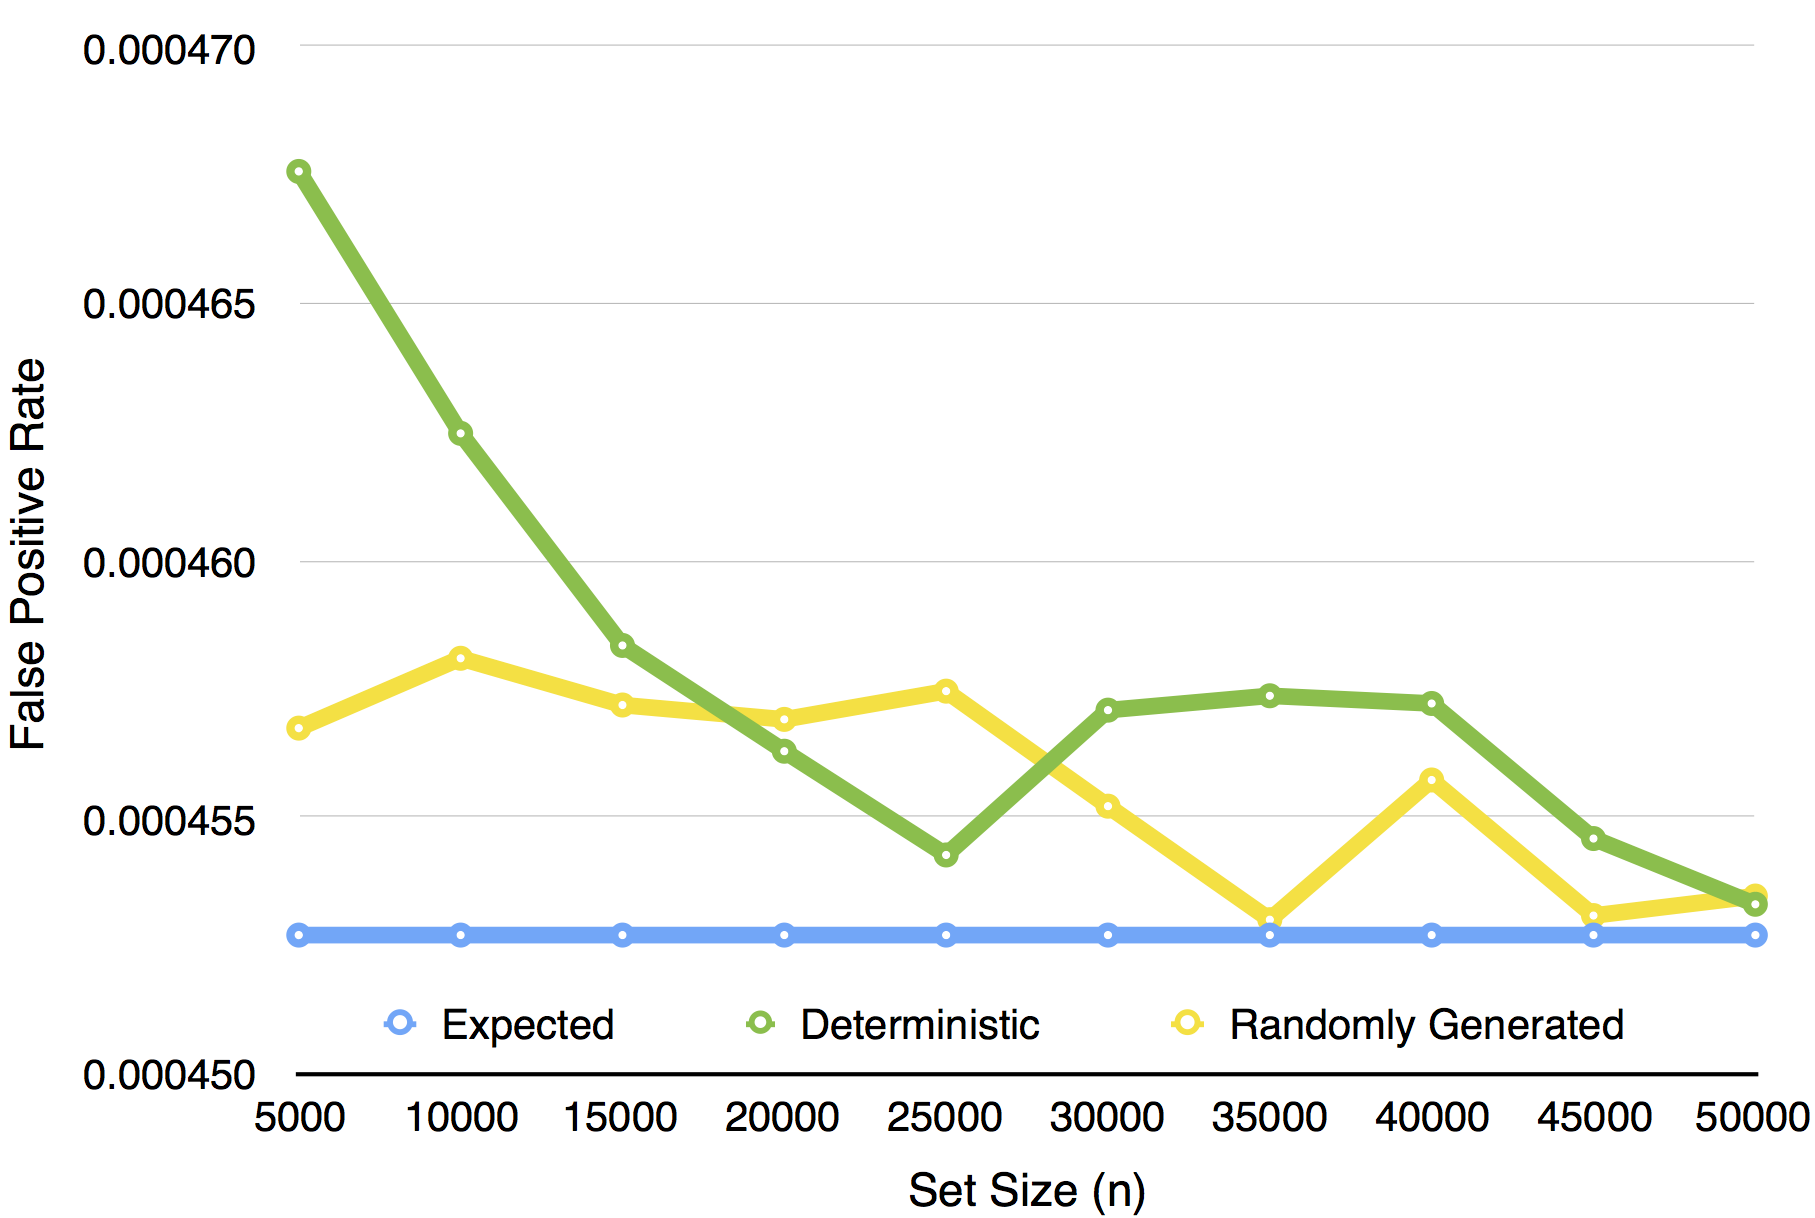
\includegraphics[width=0.5\textwidth]{figures/false_positives/b=16.png}
    }
  }

  \caption{Comparing expected and measured false positive rates of two bloom
           filter implementations when varying set size ($n$) and
           bits per element ($b$).}
\end{figure}

\begin{figure}[h]
  \makebox[\textwidth][c]{
    \subfloat[][Deterministic]{
      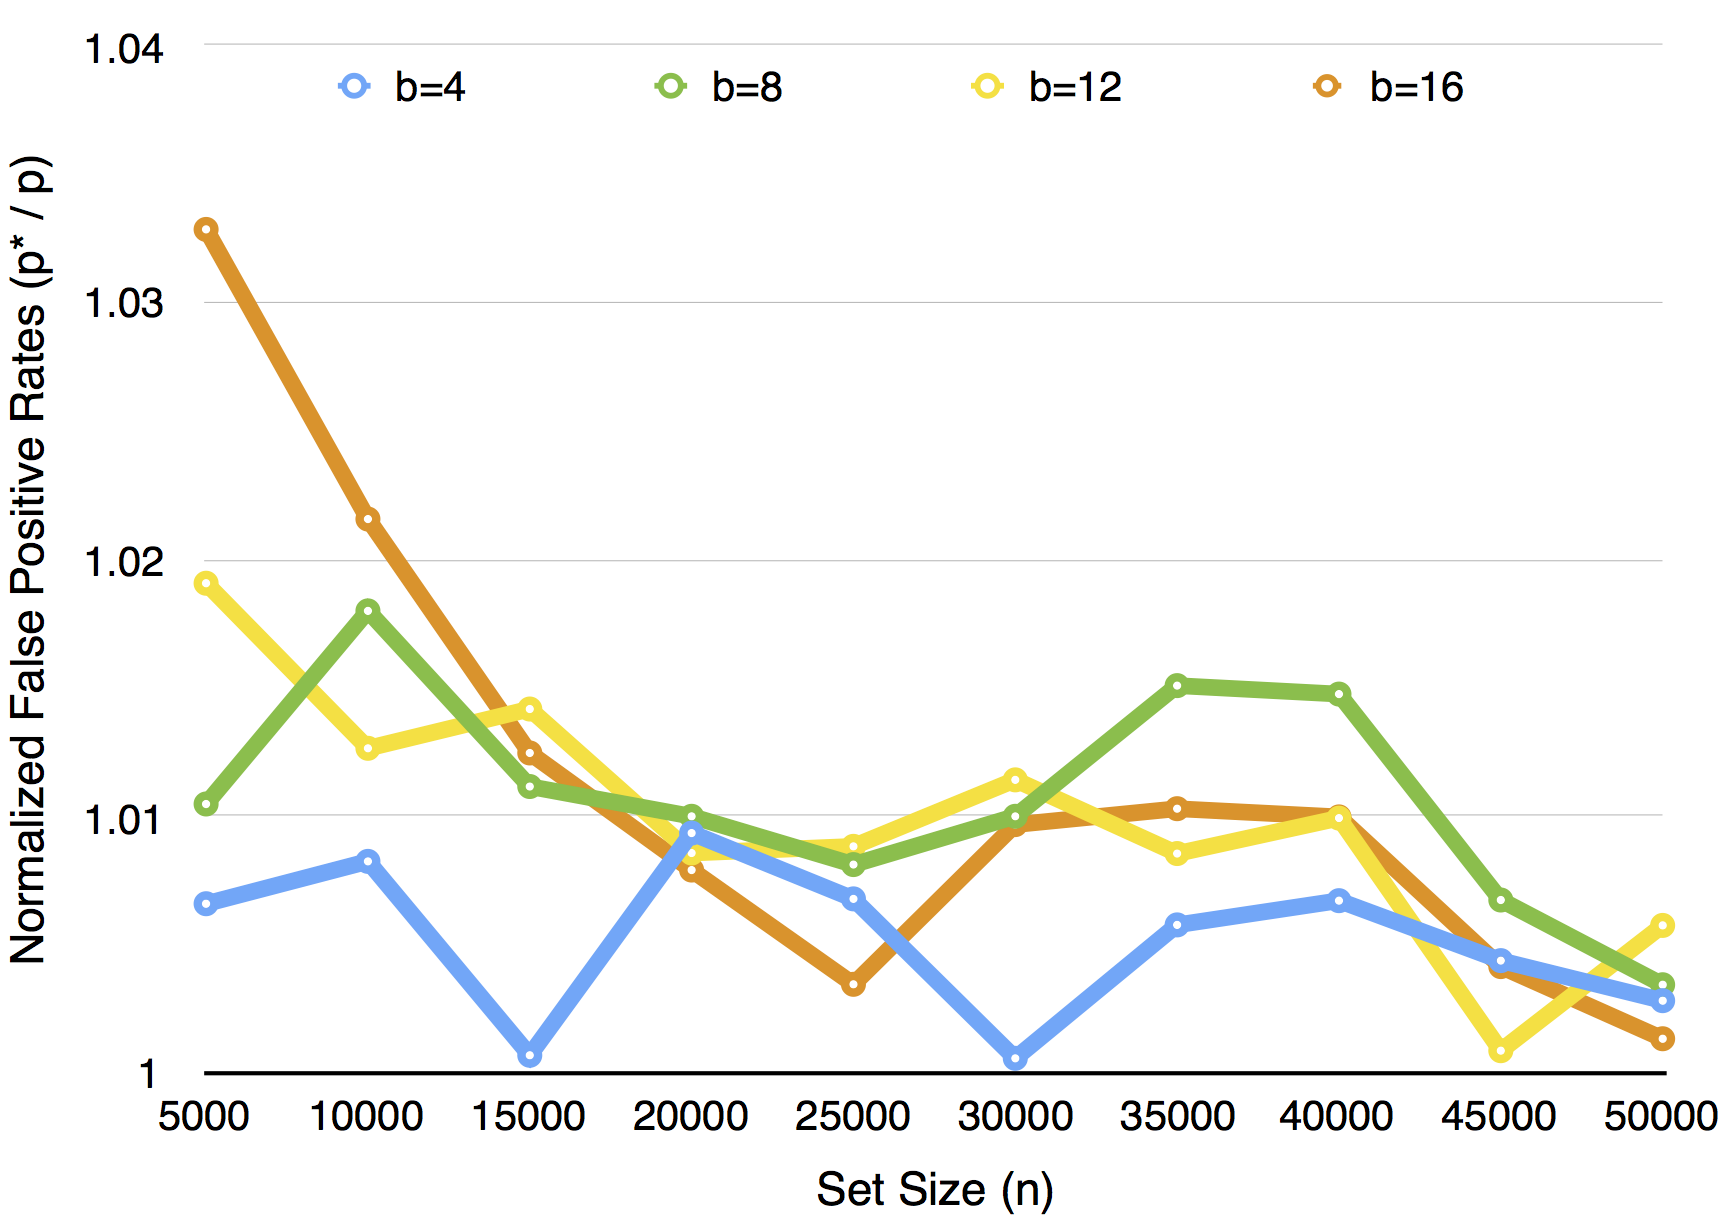
\includegraphics[width=0.5\textwidth]{figures/false_positives/normalized_deterministic.png}
    }
    \subfloat[][Randomly Generated]{
      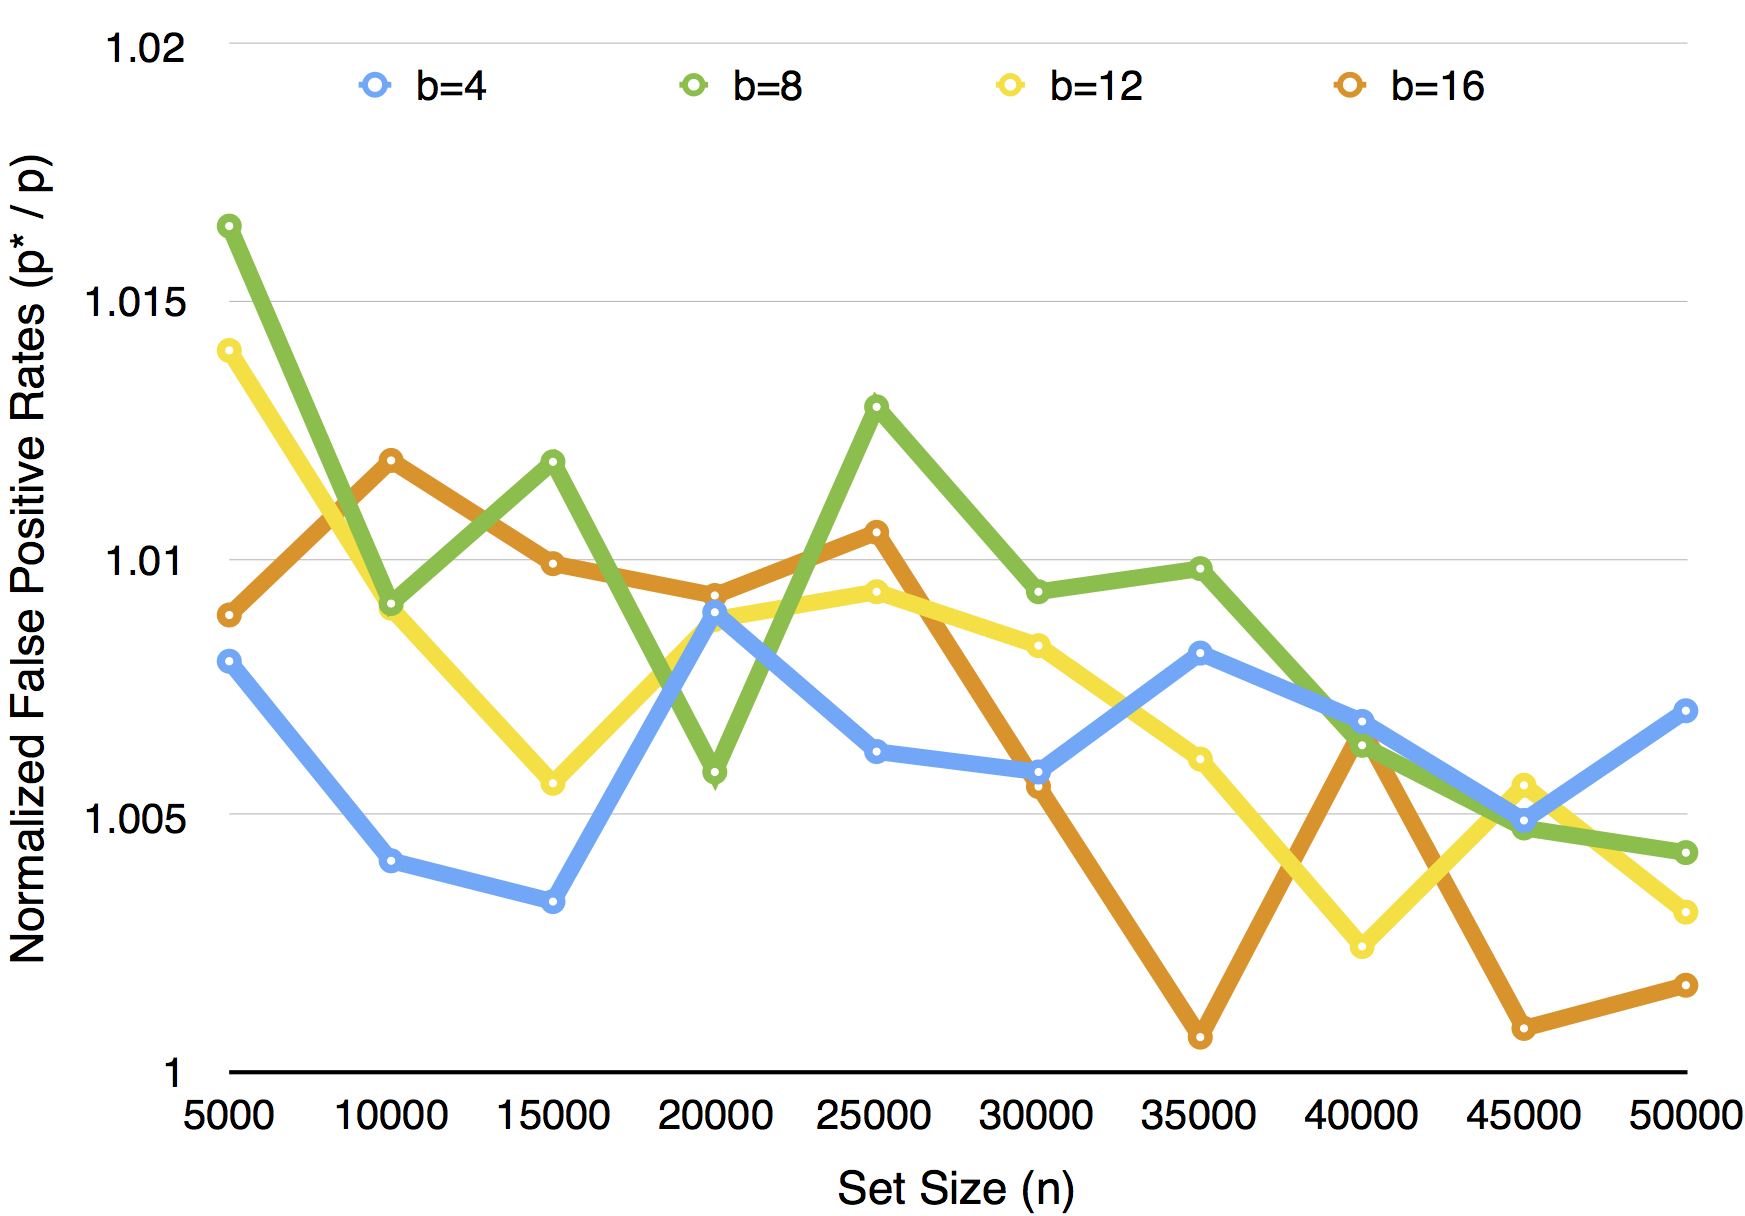
\includegraphics[width=0.5\textwidth]{figures/false_positives/normalized_random.png}
    }
  }
  \caption{Comparing normalized false positive rates when varying set size ($n$)
           and bits per element ($b$). Rates are normalized by dividing observed
           rates ($p*$) by the analytically expected rates ($p$).}
\end{figure}


\section{\texttt{EmpiricalComparison}}

\begin{figure}[h]
  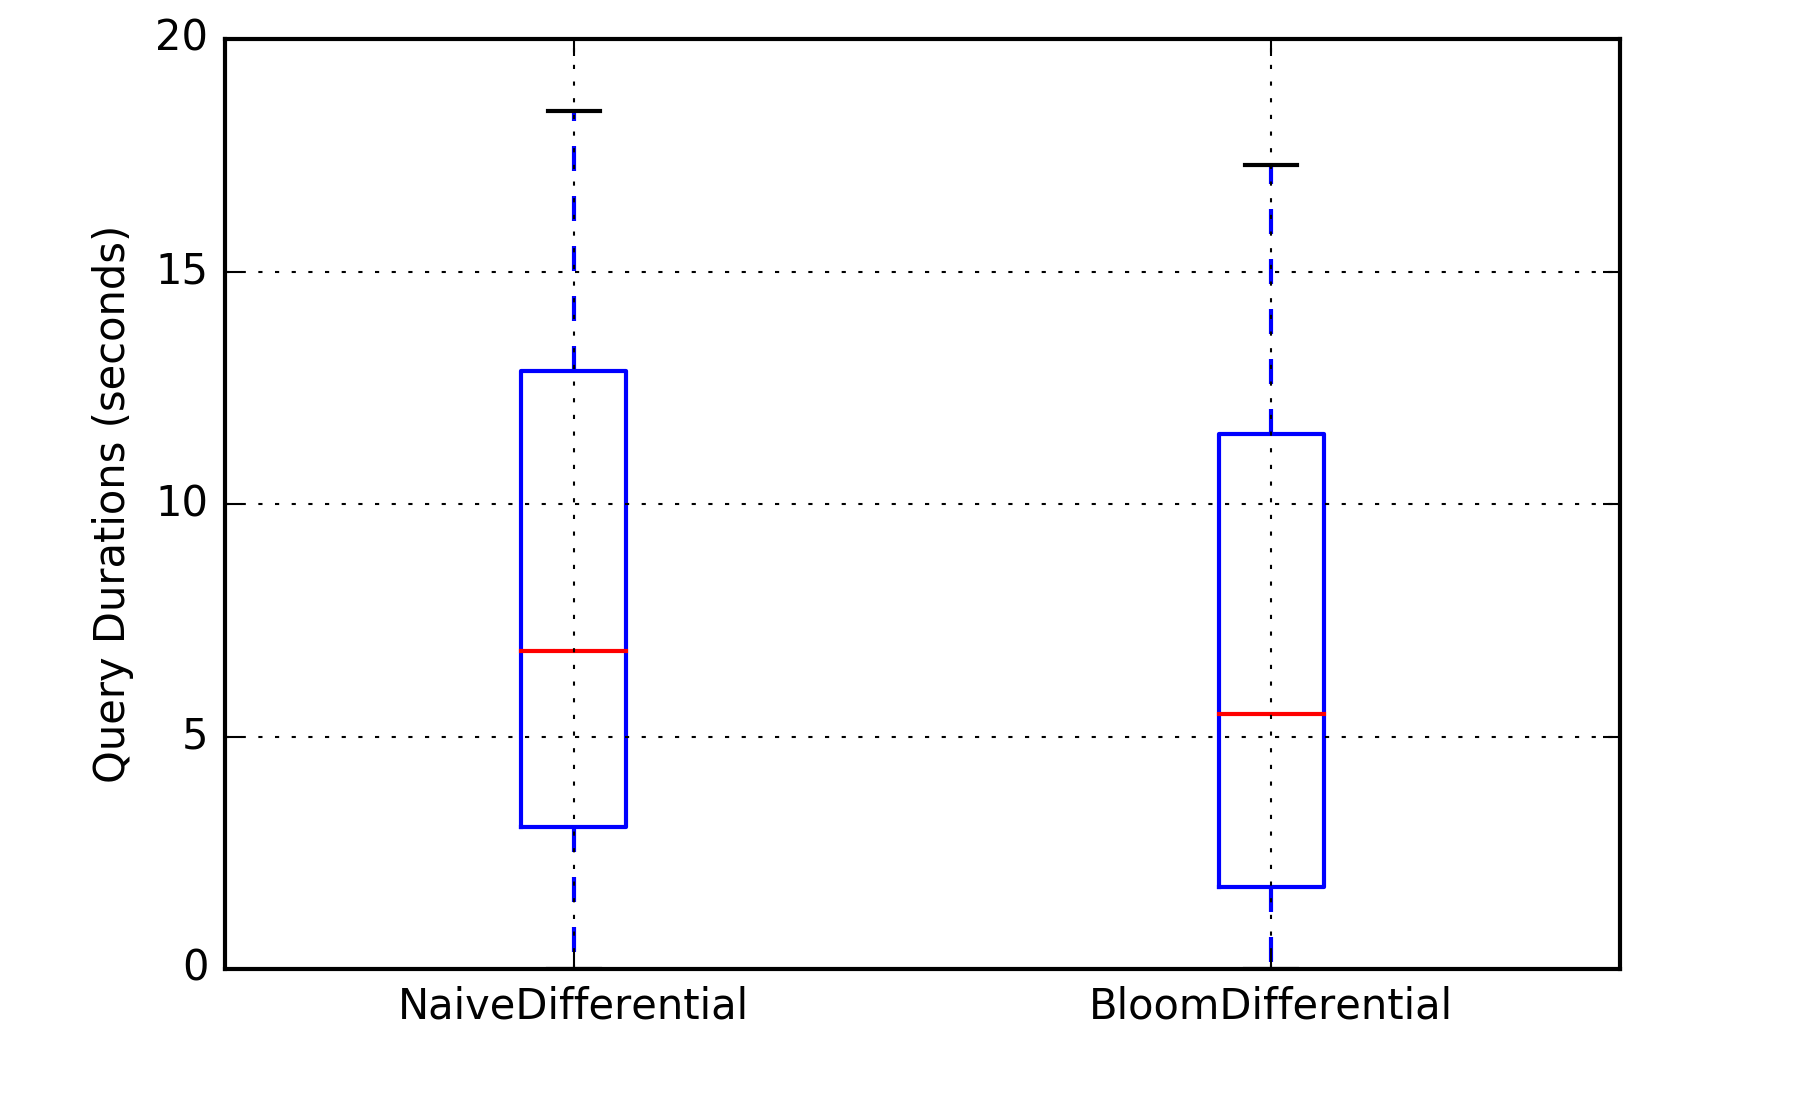
\includegraphics[width=\textwidth]{figures/empirical_comparison/query_duration_box_plot.png}
\end{figure}


\end{document}
